
\subsection{The locked invariants}
The eight-entry locked registry (F1, F4, F7, F11, F12, F18, F19, F22) is maintained as a \emph{diffable} object: the canonical declaration baseline (749 theorems / 14 definitions / 163 instances) was frozen at doctrine commit \texttt{c7c0ba17} \emph{before} the registry grew from five to eight entries, so the growth is auditable as a diff against a frozen denominator rather than a re-baseline. The three newest members of the registry are representative of the corpus's subject matter --- append-only governance data structures:
\begin{itemize}
\item \textbf{F4}: acyclicity of the governance trace DAG is preserved under append (the append operation cannot create a cycle);
\item \textbf{F7}: the FIFO batch drain admits a positional equality witness (draining a batch preserves the order in which entries were admitted);
\item \textbf{F22}: the emit log is strictly monotone (emitted sequence numbers strictly increase).
\end{itemize}
Each invariant is kernel-checked at snapshot \texttt{5cfaf9a3} and each carries the non-vacuity evidence of Figure~\ref{fig:verdict}: a bare proof term without constructor evidence is not admitted to the registry. The registry count itself is machine-checked (\texttt{locked\_count\_eight}, \texttt{by decide}) --- the paper's claim is not that the list above is complete but that the machine's count is the authority.

\subsection{Training receipts and candidate repositories}
Training-side evidence lives in dedicated receipt datasets rather than in marketing copy: \texttt{wave-logs} carries \textbf{65 genuine training logs} (real loss curves from physical runs), \texttt{szl-training-receipts} the November 5--8 training receipts, \texttt{model-eval-receipts} and \texttt{szl-frontier-evaluation-receipts} the evaluation JSONs, \texttt{energy-attested-runs} the energy attestations, and \texttt{readiness-runs} the signed daily readiness ledger. Candidate repositories (e.g., \texttt{chakana-r1}, \texttt{willay-r1/r2}, \texttt{doctrine-v2-r2}, \texttt{ouroboros-r2}, \texttt{freeenergy-r1}, \texttt{doctrine1-r1}, \texttt{abstention-v2}, \texttt{a11oy-code-r1}) hold the structured artifacts (\texttt{eval\_report.json}, \texttt{gate.heldout.jsonl}, \texttt{curriculum-manifest.json}) from which any measured card claim must quote. The estate's standing rule, learned from the incident of Section~\ref{sec:incident}: a model with no log in \texttt{wave-logs} is claimed to have \emph{no published training receipt} --- never a good one.

\section{Public Artifact Usage}
\label{sec:usage}

The only externally measured usage signal the estate publishes is download counts, read from the Hub API. The top-downloaded models at the census date:

\begin{figure}[htbp]
\centering
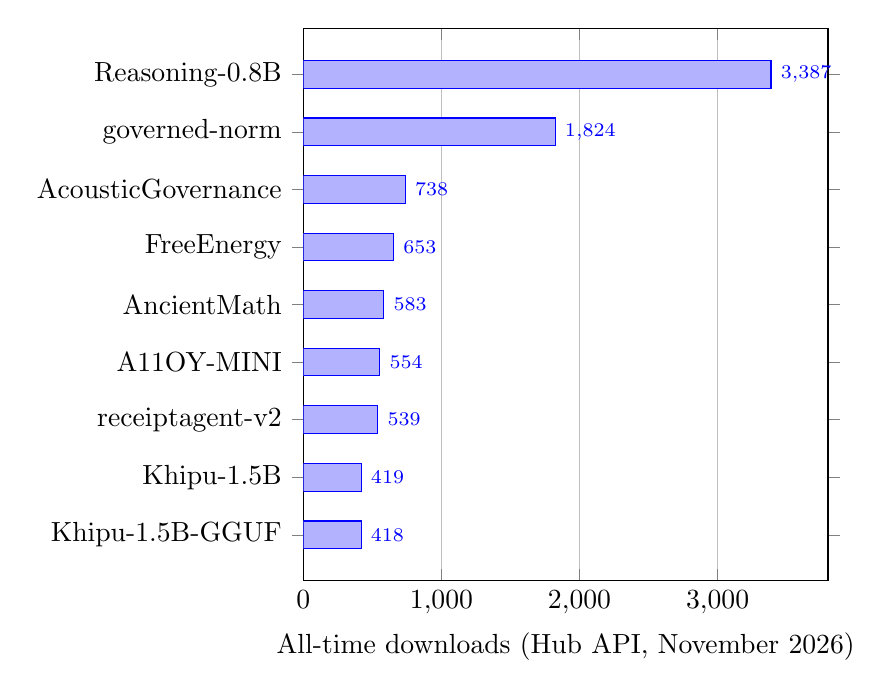
\begin{tikzpicture}
\begin{axis}[
  xbar, width=0.68\textwidth, height=8.6cm,
  symbolic y coords={R-0.8B, g-norm, Acoustic, FreeEnergy, AncientMath, A11OY-MINI, receiptagent, Khipu-1.5B, Khipu-GGUF},
  ytick=data, xmin=0, xmax=3800,
  yticklabels={Reasoning-0.8B, governed-norm, AcousticGovernance, FreeEnergy, AncientMath, A11OY-MINI, receiptagent-v2, Khipu-1.5B, Khipu-1.5B-GGUF},
  xlabel={All-time downloads (Hub API, November 2026)},
  nodes near coords, every node near coord/.append style={font=\scriptsize},
  xmajorgrids=true,
]
\addplot coordinates {(3387,Khipu-GGUF) (1824,Khipu-1.5B) (738,receiptagent) (653,A11OY-MINI) (583,AncientMath) (554,FreeEnergy) (539,Acoustic) (419,g-norm) (418,R-0.8B)};
\end{axis}
\end{tikzpicture}
\caption{Top-downloaded public models at the census date. The doctrine note is part of the measurement: \textbf{none of these repositories has a battery receipt naming it}, so no performance claim is made for any of them; download counts are the usage signal, and their graphs (where they exist) may come only from real \texttt{wave-logs}/mesh/eval receipts.}
\label{fig:downloads}
\end{figure}

\paragraph{What a download count is, and is not.} The estate publishes download counts because they are the one usage signal the Hub measures for it --- and immediately disclaims what they are not: not quality evidence, not a capability claim, not even engagement depth (a single scripted pull moves the number). The reason Figure~\ref{fig:downloads} appears in a receipt-first census at all is that its doctrine note is the measurement: the nine most-downloaded repositories have \textbf{no battery receipt naming them}, and the estate says so in the same paragraph that shows the chart. A conventional leaderboard would put the chart first and the caveat nowhere.

\paragraph{Packaging and estate surface.} Beyond the Hub, the estate publishes \textbf{21 live PyPI packages} and maintains \textbf{30 of 30 estate domains in READY state}; the x402 monetization route is live end-to-end (payable inference endpoints with the preflight fix of Section~\ref{sec:edge}). These counts are read from the same November 14--15 census that produced Figure~\ref{fig:census}; they are usage-infrastructural facts, not performance claims.

\section{Operational Timeline of the Census Window}
\label{sec:timeline}

The census window (November 13--15, 2026) was operationally dense; the estate's habit is to timestamp everything, so the window can be reconstructed from receipts. Table~\ref{tab:timeline} gives the reconstructed sequence for the incidents and repairs discussed in this paper.

\begin{table}[htbp]
\centering
\small
\begin{tabular}{lp{9.6cm}}
\toprule
\textbf{Timestamp (UTC)} & \textbf{Event} \\
\midrule
11-13 23:28 & Wave-4 trained repositories begin creation (the 31-repo set with no prior card). \\
11-14 01:16 & Correct publisher commit \texttt{1a7de2b2} lands on the Hub. \\
11-14 02:49--02:57 & Off-route stamp job overwrites 138 public cards (commits \texttt{a2b1e8df}, \texttt{1c7d1590}). \\
11-14 (day) & Fail-closed repair: 101 byte-restores (99 RESTORED, 2 CARD\_REMOVED) + 31 honest-minimal rewrites; logs \texttt{restore101\_log.jsonl}, \texttt{honest31\_log.jsonl}. \\
11-14 18:06 & A same-day edit observed on a candidate repository, logged as a parallel-publisher watch item (no action; coordination doctrine). \\
11-14 18:26 & Fleet census: 9 container groups running, 3 allocating; 4 previously crash-looping containers repatched and running by 20:46. \\
11-14 18:37 & API quota confirmed restored (4,997 calls remaining); recorded to bound the census's read reliability. \\
11-14 20:50 & Front-page lane complete: both estate front pages live end-to-end. \\
11-14 19:46 & Evening merge wave lands (a11oy main $\to$ \texttt{c7f94397}). \\
11-14 20:18--20:27 & Concurrent-push admit race diagnosed (\texttt{runtime.sha} churn); quiet-window run \texttt{43637549333} admits successfully. \\
11-14 20:27 & x402 preflight fix live: \texttt{OPTIONS} 530/1033 $\to$ 200. \\
11-14 20:34 & PR \#3421 merged (squash \texttt{0bb58a5e}). \\
11-15 02:06 & Living-anatomy guardian workflow green on main. \\
11-15 02:2x & Inference service restored on the hatun host (v7). \\
11-15 03:39 & Track A campaign closes: 143/143 attempted, 65 \texttt{sorry}-echoes, 0 empty, 0 fabrications. \\
11-15 04:39 & Battery v5 watcher exits per design (v5 manifest landed; 2 zero-scans). \\
\bottomrule
\end{tabular}
\caption{Reconstructed census-window timeline from receipted events. Every row names a receipted artifact or a commit; none is reconstructed from memory.}
\label{tab:timeline}
\end{table}

\paragraph{Parallel-lane coordination doctrine.} The window above was produced by many concurrent operator lanes on shared infrastructure, which is why the admit race of Section~\ref{sec:edge} occurred. The standing coordination doctrine is now part of the estate's operating procedure: before dispatching fixes, an operator checks the freshest file timestamps and fleet commits; findings are left as timestamped files in the shared audit directory rather than racing live lanes; and dispatch serialization through a single owner lane is the default for admit-sensitive pipelines. The doctrine is recorded here because it is an honest operational cost of the estate's velocity, not an embarrassment.

\section{Threats to Validity}
\label{sec:threats}

An honest accounting must state what could make it wrong:
\begin{enumerate}
\item \textbf{Instrument drift.} Counts differ across instruments (anonymous API vs. authenticated audit; tree-API caps). Each number in this paper names its instrument; cross-instrument comparisons are avoided rather than reconciled silently.
\item \textbf{Point-in-time sensitivity.} The estate publishes continuously; any count in this paper may be stale by the time it is read. The receipts, not the paper, are the live source of truth.
\item \textbf{Self-issued receipts.} The receipt substrate is written by the same organization whose claims it backs; it raises the cost of fabrication but cannot eliminate the possibility. External witnessing (Section~\ref{sec:limits}) is explicitly absent at publication time.
\item \textbf{Single-operator bias.} The estate is governed by one owner with agent assistance; the doctrine mitigates (fail-closed rules, merge queues, incident disclosure) but does not remove the structural risk.
\item \textbf{Negative-result selection.} The failures reported here are the ones the doctrine surfaced; unmeasured areas (marked UNKNOWN) are by definition unreported, and their size is itself unknown.
\end{enumerate}
